\chapter{Contagens aproximadas}
\label{chap:morris}


Na década de 1970, Robert Morris ~\citep{morris:78} estudou o problema de contar rapidamente \textit{trigramas} cujas 
frequências podiam chegar até 130 mil. Esses eventos eram trios de caracteres que ocorriam em textos.

O objetivo, então, era utilizar as contagens de trigramas na implementação de corretores ortográficos estátisticos 
~\citep{morris:lorinda:75} para editores de textos ~\citep{mcmahon:cherry:morris:78} que acompanhariam as distribuições 
do sistema operacional Unix dos laboratórios da Bell ~\citep{lumbroso:2018}. Contagens similares têm aplicação no 
projeto de compressores de textos estatísticos ~\citep{text:compression:1990}.

Na época, Morris utilizava um computador PDP11 da DEC com memória de 8 bits para realizar as contagens. Com 8 bits, 
somos capazes de representar ou \textit{contar} de 0 até 255. Em geral, uma memória de $n$ bits pode armazenar números 
inteiros entre 0 e $2^{n} - 1$.

Devido à limitação de espaço e ao desejo de eficiência, Morris projetou um algoritmo para realizar estimativas ou 
\textit{contagens aproximadas}, uma vez que, não era possível manter as frequências \textit{exatas} dos trigramas. Com 
seu algoritmo, Morris trouxe aleatorização e probabilidade para o centro da discussão. E para tornarmos essa discussão 
mais precisa, consideraremos o problema de determinar o número de elementos de um dado \textbf{conjunto}~$\Mbb$. 

\begin{quote}
  \textbf{Problema} \proc{ContagemAproximada($\Mbb$)}: dado um conjunto $\Mbb~=~\{ e_1, e_2, \dots, e_n \}$, encontrar 
  estimador $\hat{n}$ para o número $n$ de elementos em $\Mbb$.  
\end{quote}

Quando $\Mbb$ é conhecido de antemão, teremos um problema que é dito \textbf{estático} ou \textit{\textbf{offline}}. 
Já em problemas \textbf{dinâmicos} ou \textit{\textbf{online}}, receberemos uma sequência de operações sobre~$\Mbb$ que 
não são previamente conhecidas e devem ser realizadas uma após a outra. Entre essas operações, existirão as 
\textbf{consultas} (\textit{queries}) que podem ser, por exemplo, encontrar o número de elementos em~$\Mbb$. Teremos, 
também, as \textbf{atualizações} (\textit{updates}) que nesse capítulo, serão modificações de~$\Mbb$ somente por meio de 
inserções de elementos.

Nesse sentido, o problema estudado por Morris pode ser considerado \textbf{incremental} (não há remoções de elementos), 
e dessa forma, o conjunto $\Mbb$ pode ser visto como sendo um \textbf{fluxo} $x_1, x_2, \dots, x_t, \dots$ de elementos, 
e as consultas seriam ``Quantos elementos o conjunto $\Mbb$ possui \textbf{neste instante}~$?$`` ou 
``Quantos elementos já passaram por este fluxo``.

No entanto, estudaremos detalhadamente nesse texto, as versões estatícas dos problemas apresentados, uma vez que, as 
análises dos algoritmos que resolvem esses problemas se baseiam nessas versões. E veremos que obter a versão 
\textit{online} a partir da \textit{offline} é uma tarefa simples, e assim, as aplicações e simulações desses algoritmos 
serão baseadas em versões dinâmicas.

\section{Algoritmo de Morris}

Para armazenarmos \textit{exatamente} um valor entre $0$ e $n$, são necessários registradores com~$\Omega(\lg n)$ bits. 
Então, para que seja possível contar o número de elementos em um conjunto~$\Mbb$ com até $n$ elementos usando menos 
bits, devemos abandonar a \textit{exatidão} da contagem e buscar alternativas aceitáveis.

Morris sugeriu utilizar um contador $X$ para armazenar o valor de $\lg n$ ao invés de $n$. Neste caso, o estimador 
\textit{aproximado} $\hat{n}$ de $n$ seria~$2^{X} - 1$. Este ``-1`` na expressão faz com que essa aproximação se ajuste 
à situação em que $\Mbb = \emptyset$. E um contador como este pode ser armazenado em $O(\lg X) = O(\lg \lg n)$ bits.

A política de incremento de $X$ passa a ser a questão central do algoritmo. Morris propôs uma estratégia simples para 
realizar esse acréscimo: a cada novo elemento examinado de~$\Mbb$, o contador $X$ seria incrementado com probabilidade~ 
$2^{-X}$.

Essa estratégia pode ser vista no Algoritmo $\proc{Morris}$ cuja implementação é baseada em uma ideia da seção 
\textit{Algorithm} do artigo ~\citetitle*{ApproximateCountingAlgorithm}~\citep{ApproximateCountingAlgorithm}.Essa versão 
expressa a condição de incremento do contador como um experimento de lançamento de moedas. Sempre que um novo elemento 
do conjunto $\Mbb$ é examinado, o lançamento de $X$ moedas é simulado. O contador é incrementado somente quando os 
resultados de todos os lançamentos forem cara. E a probabilidade deste evento ocorrer é~$2^{-X}$.

O Algoritmo $\proc{Morris}$ a seguir recebe um conjunto~$\Mbb = \{ e_1, e_2, \dots, e_n \}$ e devolve um estimador~
$\hat{n}$ para $n$. Este estimador é da forma $2^{X} - 1$ em que $X$ é um número inteiro não negativo, e veremos mais 
adiante que o seu valor esperado é $n$, ou seja, $\Ebb\big(\hat{n}\big) = \Ebb\big(2^{X} - 1\big) = n$.

\begin{codebox}
  \Procname{$\proc{Morris}(\Mbb)$}
  \li $X \gets 0$
  \li \For cada $e$ em $\Mbb$ 
  \li \Do
      $r \gets \text{número de caras resultantes dos lançamentos de $X$ moedas}$ 
  \li   \If $r = 0$
  \li   \Do
          $X \gets X + 1$
        \End
      \End
  \li
  \Return $2^{X} - 1$   
  \End
\end{codebox}

Na prática, para mimetizar o lançamento de moedas, utilizamos uma função $g$ geradora de números aleatórios que recebe o
valor de $X$ e devolve um inteiro aleatório $r = g(X)$ entre 0 e $2^{X} - 1$. Este número $r$ pode ser visto como um 
inteiro de $X$ bits em que cada bit representa o resultado do lançamento de uma moeda: 0 corresponde à coroa e 1, 
à~cara. 

\begin{codebox}
  \Procname{$\proc{Morris}(\Mbb)$}
  \li $X \gets 0$                                         \label{li:morris:init}
  \li \For cada $e$ em $\Mbb$                             \label{li:morris:for:start}
  \li \Do
      $r \gets g(e)$                                      \label{li:morris:generator}
  \li   \If $r = 0$                                       \label{li:morris:increment:condition}
  \li   \Do
          $X \gets X + 1$
        \End
      \End                                                \label{li:morris:end}
  \li
  \Return $2^{X} - 1$                                     \label{li:morris:return}
  \End
\end{codebox}

\section{Qualidade da aproximação}
\label{sec:morris:analysis}
\newcommand{\morrisestimator}{\proc{Morris}(\Mbb)}

Esta seção busca investigar a qualidade do estimador devolvido pelo Algoritmo \proc{Morris} para o número $n$ de 
elementos em um dado conjunto $\Mbb$. As demonstrações apresentadas aqui são baseadas nas notas de aula de 
\citep{LectureNotesAndoni}.

Primeiro, considere que $\morrisestimator$ é o estimador devolvido pelo algoritmo tendo o conjunto $\Mbb$ como entrada. 
Note que devido às chamadas feitas ao gerador de números aleatórios $g$ na linha~$\ref{li:morris:generator}$, 
$\morrisestimator$ é uma variável aleatória. Da mesma forma, a variável~$X$ criada na linha~\ref{li:morris:init} é 
também uma variável aleatória. Esta variável é interessante para a demonstração, uma vez que, o algoritmo \proc{Morris} 
mantém a seguinte relação invariante envolvendo $X$:

\begin{quote}
  \textbf{Relação invariante} de \proc{Morris}: no início da linha~\ref{li:morris:for:start}, vale que 
  $\Ebb\big(2^{X} - 1\big) = k$, em que, $k$ é o número de elementos de $\Mbb$ já examinados. 
\end{quote}

Ao final do algoritmo, temos que $\Ebb(\morrisestimator)=\Ebb\big(2^{X}-1\big)$ e que o número de elementos de $\Mbb$ 
examinados é $n$. Assim, o seguinte teorema segue como consequência dessa relação invariante:

\begin{theorem}[do valor esperado de $\morrisestimator$]
  \label{morris:theorem:expected_value}
  Se $\Mbb$ é um conjunto com $n$ elementos, então $\Ebb(\morrisestimator) = n$.
\end{theorem}

Denotemos por $X_k$ como sendo o valor da variável $X$ na linha~\ref{li:morris:for:start} após $k$ elementos de~$\Mbb$ 
terem sido examinados no laço das linhas~\ref{li:morris:for:start}--\ref{li:morris:end}. Inspecionaremos o valor de 
$\Ebb\big(2^{X_k} - 1\big)$ para alguns valores específicos de $k$ antes de passarmos para a demonstração da relação 
invariante.

Quando nenhum elemento de $\Mbb$ foi processado, o valor da variável $X$ é igual ao seu valor inicial e dessa maneira,
$X_0 = 0$. Segue que
\[ \Ebb\big(2^{X_0} - 1\big) = \Ebb\big(2^0 - 1\big) = E(0) = 0 \ .\]

Na primeira iteração do laço das linhas~\ref{li:morris:for:start}--\ref{li:morris:end}, temos que $r = g(0) = 0$ e 
consequentemente, $X_1 = 1$. Dessa forma, 
\[ \Ebb\big(2^{X_1} - 1\big) = \Ebb\big(2^1 - 1\big) = E(1) = 1 \ .\]

A determinação de $\Ebb(2^{X_2} - 1)$ é mais desafiadora. A partir deste ponto, é interessante explicitarmos a relação
de recorrência geral de $X_k$:
\begin{align}
  \label{morris:rec:xk}
X_k = \begin{cases} 
  0                 & \mbox{se } k = 0 \\[2mm]
  X_{k-1}           & \mbox{se } g(X_{k-1}) \neq 0 \\[2mm]
  X_{k-1} + 1       & \mbox{se } g(X_{k-1}) =  0\ .  
\end{cases}
\end{align}
A relação acima é decorrente das linhas~\ref{li:morris:for:start}--\ref{li:morris:end}. Na $k$-ésima iteração deste 
laço, a condicional da linha~\ref{li:morris:increment:condition} garante que o valor de $X_k$ será $X_{k-1} + 1$ se o 
número $r$ gerado na linha~\ref{li:morris:generator} for~zero. A probabilidade deste evento ocorrer é 
$\Pbb(g(X_{k-1}) = 0) = 1/2^{X_{k-1}}$, uma vez que, $r$ é um número aleatório escolhido uniformemente 
entre~$0$~e~$2^{X_{k-1}} - 1$, inclusive. Nesse sentido, a probabilidade de o valor de $X_k$ ser $X_{k - 1}$ é igual ao 
complementar de $\Pbb(g(X_{k-1}) = 0)$ e assim, 
\[\Pbb(g(X_{k-1}) \not\eq 0) = 1 - \Pbb(g(X_{k-1}) = 0) = 1 - 1/2^{X_{k-1}} \ . \]

Podemos, agora, obter a partir da recorrência~\eqref{morris:rec:xk}, uma expressão \textit{recursiva} para os valores de 
$2^{X_k} - 1$ para $k = 0,1,2,\dots$.
\begin{align}
  \label{morris:rec:2xk}
  2^{X_k}-1 = \begin{cases} 
  0                     & \mbox{se } k = 0 \\[2mm]
  2^{X_{k-1}} - 1       & \mbox{se } g(X_{k-1}) \neq 0 \\[2mm]
  2^{X_{k-1} + 1} - 1   & \mbox{se } g(X_{k-1}) =  0\ .  
\end{cases}
\end{align}
E com a recorrência~\eqref{morris:rec:2xk} e os valores de $\Pbb(g(X_{k-1}) = 0)$ e $\Pbb(g(X_{k-1}) \not\eq 0)$, 
podemos encontrar uma expressão para $\Ebb\big(2^{X_k} - 1\big)$:
\begin{align}
  \label{morris:rec:e}
  \Ebb\big(2^{X_k} - 1\big)
  &= \Ebb \Big( \ \underbrace{\Big(1 - \frac{1}{2^{X_{k-1}}}\Big)}_{\Pbb( \ g(X_{k-1}) \ \not\eq \ 0 \ )} \ \times \
  \Big( 2^{X_{k-1}}-1 \Big) + \underbrace{\frac{1}{2^{X_{k-1}}}}_{\Pbb( \ g(X_{k-1}) \ = \ 0 \ )} \ \times \
  \Big(2^{X_{k-1} + 1} - 1 \Big) \ \Big) \nonumber \\[2mm]
  &= \Ebb\Big(\ 2^{X_{k-1}} - 1 - \frac{2^{X_{k-1}}}{2^{X_{k-1}}} + \frac{1}{2^{X_{k-1}}}  + 
  \frac{2^{X_{k-1} + 1}}{2^{X_{k-1}}}  - \frac{1}{2^{X_{k-1}}} \ \Big) \nonumber \\[2mm]
  & = \Ebb\Big(\ 2^{X_{k-1}} - 1 - 1 + \frac{1}{2^{X_{k-1}}}  + 2  - \frac{1}{2^{X_{k-1}}} \ \Big) \nonumber \\[2mm]
  & = \Ebb\big( 2^{X_{k-1}}  \big) \ .
\end{align}
E tomando $k = 2$ nesta expressão, obtemos
\begin{align*}
  \Ebb\big(2^{X_2}-1\big) & =  \Ebb\big(2^{X_{2-1}}\big) = \Ebb\big(2^{X_{1}}\big) = \Ebb\big(2^{{1}}\big) = 2 \ . 
\end{align*}

Os cálculos envolvidos na determinação de $\Ebb\big(2^{X_3} - 1\big)$ estão explicitados na árvore de decisão da 
Figura~\ref{fig:morris-tree}. Nesta árvore, podemos encontrar os possíveis valores para as variáveis aleatórias $X_1$, 
$X_2$ e $X_3$, além das probabilidades de cada variável assumir um certo valor. As setas da cor verde indicam que o 
contador foi incrementado e as da cor vermelha, que o contador não sofreu mudanças. Assim, para que tenhamos, por 
exemplo, $X_3 = 3$, é necessário que durante as iterações do algoritmo, obtenhamos $g(1) = 0$ e $g(2) = 0$. Este evento 
ocorre com probabilidade $1/2 \times 1/4 = 1/8$. Na figura, este fato é indicado com a fração $1/8$ próxima à folha de 
rótulo $X_3 = 3$.

\begin{figure}
  \centering
  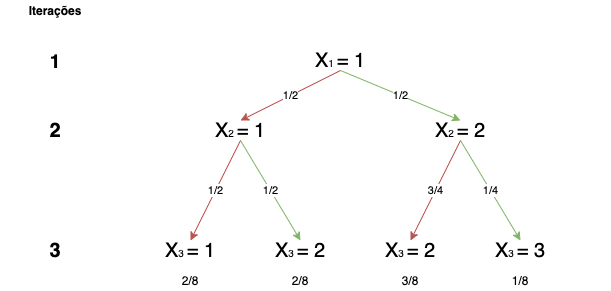
\includegraphics[scale=0.50]{figuras/morris-tree.png}
	\caption{Árvore de decisão para determinar $\Ebb\big(2^{X_3} - 1\big)$ no algoritmo \proc{Morris}. A fração próxima de 
  cada folha indica a probabilidade de $X_3$ assumir o valor em seu rótulo.}\label{fig:morris-tree}

\end{figure}

Inspecionando as folhas da árvore acima, vemos que
\begin{align*}
  \Ebb\big(2^{X_3} - 1\big) 
    &=  \frac{2}{8} \times \big(2^1 - 1\big) + \frac{2}{8} \times \big(2^2 - 1\big) + \frac{3}{8} \times 
        \big(2^2 - 1\big) + \frac{1}{8} \times \big(2^3 - 1\big) \\
    &= \frac{2}{8} \times 1 + \frac{2}{8} \times 3 + \frac{3}{8} \times 3 + \frac{1}{8} \times 7 \\
    &= \frac{24}{8} \\
    &= 3 \ .
\end{align*}

Em todos os exemplos calculados até agora, vimos que $\Ebb\big(2^{k} - 1\big) = k$. Após ganharmos intuição sobre
$\Ebb\big(2^{k} - 1\big)$ com valores pequenos de $k$, estamos preparados para demonstrar a validade da relação 
invariante.

\begin{proof}[Demonstração \ (da relação invariante)]
  A prova será por indução no número $k$ de elementos de $\Mbb$ já examinados. Vimos anteriormente que 
  $\Ebb\big(2^0 - 1 \big) = 0$ e asssim, a relação vale para $k = 0$.

  Suponhamos, agora, que a relação invariante vale para algum $k - 1$, $k \geq 1$. Mostraremos que isso implica que esta
  relação vale para $k$. Dessa forma, temos que

  \begin{align}
      \Ebb\big(2^{X_k} - 1\big) 
      &= \Ebb\big(2^{X_{k-1}}\big)  \label{proof:morris:01}  \\
      &= \Ebb\big(2^{X_{k-1}}\big) - 1 + 1 \nonumber \\
      &= \Ebb\big(2^{X_{k-1}} - 1\big) + 1 \nonumber \\
      &= k - 1 + 1 \label{proof:morris:02} \\ 
      &= k \nonumber,
    \end{align}    

    em que a igualdade~\eqref{proof:morris:01} é decorrência da identidade~\eqref{morris:rec:e} e a 
    igualdade~\eqref{proof:morris:02}, da hipótese de indução. Finalmente, a validade da relação invariante segue do 
    princípio da indução finita.
\end{proof}  

Saber que $\Ebb(\proc{Morris}(\Mbb)) = |\Mbb| = n$ não é suficiente para garantir a qualidade do estimador $2^{X} - 1$
devolvido pelo algoritmo. É desejável que além do valor esperado ser próximo ou igual ao tamnho do conjunto $\Mbb$, que
a variância da variável aleatória \proc{Morris}($\Mbb$) não seja \textit{muito grande}. Intuitivamente, isso nos diria 
que a probabilidade do estimador calculado ser longe do valor esperado é pequena. Então, apresentaremos o valor da 
variância de $\proc{Morris}(\Mbb)$ no próximo teorema.

\begin{theorem}[da variância]
  \label{morris:theorem:variance}
  Se $\Mbb$ é um conjunto com $n$ elementos, então $\Vbb(\Ebb(\morrisestimator)) = n(n - 1) / 2$.
\end{theorem}

\begin{proof}[Demonstração \ (da variância)]
  Pela definição da \hyperref[ap:variance]{variância} de uma variável aleatória, temos que

  \begin{align}
    \Vbb(\proc{Morris}(\Mbb))
    &= \Ebb(\proc{Morris}(\Mbb)^2) - \Ebb^2(\proc{Morris}(\Mbb)) \nonumber \\ 
    &= \Ebb\big(\big(2^{X_n} - 1\big)^2\big) - n^2 \label{proof:morris:var:01} \\
    &= \Ebb\big(2^{2X_n} - 2\big(2^{X_n}\big) + 1\big) - n^2 \nonumber \\
    &= \Ebb\big(2^{2X_n}\big) - 2\Ebb\big(2^{X_n}\big) + 2 - 2 + 1 - n^2 \nonumber \\
    &= \Ebb\big(2^{2X_n}\big) - 2\Ebb\big(2^{X_n} - 1\big) - 2 + 1 - n^2 \nonumber \\
    &= \Ebb\big(2^{2X_n}\big) - 2n - 1 - n^2 \label{proof:morris:var:02} \ ,
  \end{align}

  em que utilizamos a identidade $\Ebb(\proc{Morris}(\Mbb)) = \Ebb\big(2^{X_n} - 1\big) = n$ nas igualdades~
  \eqref{proof:morris:var:01}~e~\eqref{proof:morris:var:02}.

  Logo em seguida, passaremos a calcular $\Ebb\big(2^{2X_n}\big)$. Para isso, procederemos de maneira idêntica ao que 
  foi feito na demonstração do Teorema~\hyperref[morris:theorem:expected_value]{do valor esperado} utilizando a 
  recorrência~\eqref{morris:rec:xk}. Assim,

  \begin{align}
    \Ebb\big(2^{2X_n}\big)
    &=  \Ebb\Big(\Big(1 - \frac{1}{2^{X_n}}\Big) \times 2^{2X_{n - 1}} + \frac{1}{2^{X_n}} \times 2^{2(X_{n-1} 
        + 1)}\Big) \nonumber \\
    &=  \Ebb\bigg(2^{2X_{n-1}} - \frac{2^{2X_{n-1}}}{2^{X_{n-1}}} + \frac{2^{2(X_{n-1}+1)}}{2^{X_{n-1}}}\bigg) 
        \nonumber \\
    &= \Ebb\big(2^{2X_{n-1}} -2^{X_{n-1}} + 2^{X_{n-1}+2}\big) \nonumber \\
    &= \Ebb\big(2^{2X_{n-1}} + 3 \times 2^{X_{n-1}}\big) \nonumber \\
    &= \Ebb\big(2^{2X_{n-1}}\big) + 3\Ebb\big(2^{X_{n-1}}\big) \label{proof:morris:var:03} \\
    &= \Ebb\big(2^{2X_{n-1}}\big) + 3n  \ . \nonumber
  \end{align}

  A igualdade~\eqref{proof:morris:var:03} segue da identidade~\eqref{morris:rec:e}. E o valor de 
  $\Ebb\big(2^{2X_n}\big)$ pode ser obtido da expansão \textit{telescópica} da relação de recorrência

  \begin{align*}
    \Ebb\big(2^{2X_n}\big)
    &= \Ebb\big(2^{X_{n-1}}\big) + 3n \\
    &=  \Ebb\big(2^{X_{n-2}}\big) + 3(n - 1) + 3n \\
    &=  \Ebb\big(2^{X_{n-3}}\big) + 3(n - 2) + 3(n - 1) + 3n \\
    &\hspace{5mm} \vdots\\
    &=1 + 3 + \dots + 3(n-2) + 3(n-1) + 3n \\
    &=\frac{3n(n+1)}{2} + 1 \ .
  \end{align*}

  Finalmente, utilizando esse valor para prosseguir com \eqref{proof:morris:var:02}, obtemos

  \begin{align*}
    \Vbb(\proc{Morris}(\Mbb))
    &= \Ebb\big(2^{2X_n}\big) - 2n - 1 - n^2 \\
    &= \frac{3n(n+1)}{2} + 1 - 2n -1 -n^2 \\
    &= \frac{3n(n+1) - 4n - 2n^2}{2} \\
    &= \frac{n(n-1)}{2} \ .
  \end{align*}

\end{proof}

Dessa forma, podemos estimar o erro do algoritmo \proc{Morris} a partir dos Teoremas 
\hyperref[morris:theorem:expected_value]{do valor esperado} e \hyperref[morris:theorem:variance]{da variância}. Seja
$\sigma$ o desvio padrão de \proc{Morris}($\Mbb$). A \hyperref[ap:chebyshev]{desigualdade de Cherbyshev} nos diz que 
para todo $c > 0$, 
\begin{align}
  \Pbb(|\proc{Morris}(\Mbb) - n| \geq c\sigma) \leq \frac{1}{c^2} \ .  \label{morris:error}
\end{align}

Pondo $c = 4\sqrt{2}$ em \eqref{morris:error}, obtemos que 
\begin{align}
  \Pbb\big(|\proc{Morris}(\Mbb) - n| \geq 4\sqrt{2} \times \sigma\big) \leq \frac{1}{(4\sqrt{2})^2} = \frac{1}{32} \ .
\end{align}

Como pelo Teorema \hyperref[morris:theorem:variance]{da variância},
\[ \sigma^2 = \Vbb(\proc{Morris}(\Mbb)) = \frac{n(n-1)}{2} \ , \] vale que
\[ \sigma < \frac{n}{\sqrt{2}} \ . \]

Logo, temos que
\[  \Pbb\bigg(|\proc{Morris}(\Mbb) - n| \geq 4\sqrt{2} \times \frac{2}{\sqrt{2}}\bigg) =  
    \Pbb(|\proc{Morris}(\Mbb) - n| \geq 4n) \leq \frac{1}{32} \ . \]
    
Portando, podemos concluir que 
\begin{align}
  \Pbb(|\proc{Morris}(\Mbb) - n| \geq 4n) \leq \frac{1}{32} < 0{,}032 \ .  \label{morris:error:result}
\end{align}

Em palavras, isto nos diz que com probabilidade maior que $96{,}8\%$, o erro relativo cometido por \proc{Morris}($\Mbb$) 
é menor do que 4.

Por fim, voltemos nossa atenção para uma das motivações iniciais do trabalho de Morris: o espaço utilizado pelo 
algoritmo. Por espaço, queremos dizer o número de bits que o algoritmo \proc{Morris} necessita para representar o 
contador~$X$ definido na linha~\ref{li:morris:init}. Denotaremos por \proc{bits}($i$) como sendo o menor número de bits
para representar um número inteiro não-negativo $i$. Temos que \proc{bits}(0) = 1 e para $i \geq 1$, \proc{bits}($i$) = 
$\lfloor\lg i\rfloor + 1$.

\begin{theorem}
  \label{morris:theorem:space}
  Sejam $\Mbb$ um conjunto com $n \geq 2$ elementos, $X$ a variável definida na linha~\ref{li:morris:init} do algoritmo
  \proc{Morris} e $b$ um número inteiro positivo. Se $X_n$ é o valor da variável~$X$ ao final de \proc{Morris}($\Mbb$), 
  então $\Pbb(\proc{bits}(X_n) \geq b + \lg\lg n + 1) \leq 1/(n^{2^b-1}-1)$.
\end{theorem}

Consideremos um exemplo para decifrar o significado do Teorema~\ref{morris:theorem:space}. Suponhamos que $\Mbb$ é um 
conjunto com $n = 2^{16} = 65536$ elementos. Neste caso, temos que $\lg \lg n = 4$. O teorema nos diz que para $b = 1$,
a representação de $X = X_{65536}$ utilizará 6 bits com probabilidade menor ou igual a 
$1/(65536^{2^1 - 1}) = 1/65536 < 1{,}53 \times 10^{-5}$. E para $b = 2$, seriam necessários 7 bits com probabilidade 
menor ou igual a $1/(65536^{2^2 - 1}) < 3{,}56 \times 10^{-15}$. Nesse sentido, o Teorema~\ref{morris:theorem:space} nos 
garante que o algoritmo \proc{Morris} consome \textit{quase certamente} não mais que $\lceil\lg \lg n\rceil$ bits de 
espaço.

\begin{proof}[Demonstração \ (do Teorema~\ref{morris:theorem:space})]
  A \hyperref[ap:markov]{desigualdade de Markov} nos diz que para todo número real positivo $c$ vale que
  \begin{align}
    \Pbb(\proc{Morris}(\Mbb) \geq c) \leq \frac{\proc{Morris}(\Mbb)}{c} = \frac{n}{c} \ . \label{morris:markov}
  \end{align}
  Pondo $c = n^{2^b} - 1$ em \eqref{morris:markov}, obtemos que
  \begin{align}
    \Pbb\big(\proc{Morris}(\Mbb) \geq n^{2^b} - 1\big) \leq \frac{1}{n^{2^b-1} - 1} \ . \label{morris:memory:step}
  \end{align}
  Como $\proc{Morris}(\Mbb) = 2^{X_n} - 1$, reescrevendo e desenvolvendo \eqref{morris:memory:step}, encontramos que
  \begin{align*}
    \Pbb\big(2^{X_n} - 1 \geq n^{2^b} - 1\big)
    &=  \Pbb\big(2^{X_n} \geq n^{2^b}\big) \\
    &=  \Pbb\big(X_n \geq \lg n^{2^b}\big) \\
    &=  \Pbb\big(\lg X_n \geq \lg \lg n^{2^b}\big) \\
    &\geq  \Pbb\big(\lfloor\lg X_n\rfloor \geq \lg \lg n^{2^b}\big) \\
    &=  \Pbb\big(\lfloor\lg X_n\rfloor + 1 \geq \lg \lg n^{2^b} + 1\big) \\
    &=  \Pbb\big(\proc{bits}(X_n) \geq \lg \lg n^{2^b} + 1\big) \\
    &=  \Pbb\big(\proc{bits}(X_n) \geq \lg 2^{b} + \lg \lg n + 1\big) \\
    &=  \Pbb(\proc{bits}(X_n) \geq b + \lg \lg n + 1) \ .
  \end{align*}
  Combinando a desigualdade acima com \eqref{morris:memory:step}, vemos que
  \[  \Pbb(\proc{bits}(X_n) \geq b + \lg \lg n + 1) \leq \frac{1}{n^{2^b-1} - 1} \ . \]
  Com isto, concluímos a prova do teorema.
\end{proof}

\section{\proc{Morris} e a lei dos grandes números}
\label{sec:morris:plus}

Do teorema \hyperref[morris:theorem:variance]{da variância de \proc{Morris}($\Mbb$)}, notamos que o algoritmo apresenta
uma grande variabilidade. Nesta seção, veremos uma técnica que a partir de um algoritmo probabilístico com uma certa 
variância, obteremos um novo algoritmo com variância menor.

Em nosso caso, nos apoiaremos no algoritmo \proc{Morris} para construir o algoritmo \proc{Morris++} que tem o mesmo 
valor esperado e menor variância que \proc{Morris}. Como foi visto em \eqref{morris:error}, a desigualdade de Cherbyshev
limita o erro em função da variância, e assim, o erro relativo de \proc{Morris++} também será menor que o de 
\proc{Morris}. E as demonstrações apresentadas aqui serão também baseadas nas notas de aula 
de~\citep{LectureNotesAndoni}.

O algoritmo \proc{Morris++} recebe um conjunto $\Mbb = \{ e_1, e_2, \dots, e_n \}$ e um número positivo~$t$, e devolve 
um estimador~$\hat{n}$ para $n$. Este estimador será a média aritmética de $t$ execuções de \proc{Morris}($\Mbb$). Esta 
estratégia é inspirada na \proc{Lei dos Grandes Números}, que diz que a média dos resultados obtidos de um grande número 
de experimentos deve se aproximar do valor esperado à medida que mais experimentos são realizados.

\begin{codebox}
  \Procname{$\proc{Morris++}(\Mbb, t)$}
  \li $N \gets 0$                       \label{prog:morris:plus:start}                
  \li \For $i \gets 1$ até $t$                             
  \li \Do
      $n_i \gets \proc{Morris}(\Mbb)$   \label{prog:morris:plus:n}
  \li $N \gets N + n_i$
      \End
  \li
  \Return N/t
  \End
\end{codebox}

As variáveis $n_1, n_2, \dots, n_t$ definidas na linha~\ref{prog:morris:plus:n} são aleatórias e tais que
\begin{align}
  \Ebb(n_i) &= \Ebb(\proc{Morris}(\Mbb)) = n                \label{morris:plus:n:exp} \\     
  \Vbb(n_i) &= \Vbb(\proc{Morris}(\Mbb)) = n(n - 1)/2 \ ,   \label{morris:plus:n:var}
\end{align}

para $i = 1, 2, \dots, t$. A igualdade~\eqref{morris:plus:n:exp} é decorrência do teorema 
\hyperref[morris:theorem:expected_value]{do valor esperado de \proc{Morris}($\Mbb$)}, e a igualdade~
\eqref{morris:plus:n:var}, do teorema \hyperref[morris:theorem:variance]{da variância de \proc{Morris}($\Mbb$)}.

De maneira semelhante ao que já havíamos feito, denotaremos por $\proc{Morris++}(\Mbb, t)$ como sendo o estimador 
devolvido pelo algoritmo tendo o conjunto $\Mbb$ e o número inteiro $t$ como entrada. É evidente que 
$\proc{Morris}(\Mbb) = \proc{Morris++}(\Mbb, 1)$.

\begin{theorem}[do valor esperado de $\proc{Morris++}$]
  \label{morris:plus:expected_value}
  Se $\Mbb$ é um conjunto com $n$ elementos e $t$, um número inteiro positivo, então 
  $\Ebb(\proc{Morris++}(\Mbb, t)) = n \ .$
\end{theorem}

\begin{proof}[Demonstração]
  \label{demo:morris:plus}
  A variável aleatória $N$ é definida na linha~\ref{prog:morris:plus:start}. Seja $N_t$ o valor desta variável ao final 
  da execução do algoritmo. Temos que

  \begin{align}
    \Ebb\big(\proc{Morris++}(\Mbb,t)\big)
    &= \Ebb\bigg(\frac{N_t}{t} \bigg)  \nonumber\\
    &= \Ebb\bigg(\frac{n_1 + n_2 + \dots + n_t}{t} \bigg)  \nonumber\\
    &= \frac{\Ebb(n_1) + \Ebb(n_2) + \dots + \Ebb(n_t)}{t}  \nonumber\\
    &= \frac{\Ebb(\proc{Morris}(\Mbb)) + \dots + \Ebb(\proc{Morris}(\Mbb))}{t}  \label{demo:morris:plus:exp:01} \\
    &= \frac{1}{t} \times t \times \Ebb(\proc{Morris}(\Mbb)) \nonumber\\
    &= \Ebb(\proc{Morris}(\Mbb)) \nonumber\\
    &= n \ ,  \label{demo:morris:plus:exp:02}
  \end{align}

  em que as igualdades em \eqref{demo:morris:plus:exp:01} e \eqref{demo:morris:plus:exp:02} seguem das identidades 
  em~\eqref{morris:plus:n:exp}.
\end{proof}

\begin{theorem}[da variância de $\proc{Morris++}$]
  \label{morris:plus:variance}
  Se $\Mbb$ é um conjunto com $n$ elementos e $t$ é um número inteiro positivo, então 
  $\Vbb(\Morrispp(\Mbb,t)) = \Vbb(\Morris(\Mbb))/t = n(n-1)/2t\ . $
\end{theorem}

\begin{proof}
  Retome a definição de $N_t$ na \hyperref[demo:morris:plus]{demonstração do valor esperado}. Temos que

  \begin{align}
    \Vbb\big(\Morrispp(\Mbb,t)\big) & = \Vbb\bigg(\frac{N_t}{t}\bigg) \nonumber\\
    & = \Vbb\bigg(\frac{n_1 + n_2 + \dots +n_t}{t} \bigg) \nonumber\\
    &= \frac{1}{t^2} \times \Vbb(n_1 + n_2 + \dots + n_t)  \nonumber\\
    &= \frac{1}{t^2} \times \bigg(\sum_{i=1}^t\Vbb(n_i) + 2\times \sum_{i<j}\Cov(n_i,n_j)\bigg)\\
    &= \frac{1}{t^2} \times \sum_{i=1}^t\Vbb(n_i) \label{demo:morrs:plus:var:01}\\
    &= \frac{1}{t^2} \times \sum_{i=1}^t\Vbb(\Morris(\Mbb)) \label{demo:morris:plus:var:02} \\
    &= \frac{1}{t^2} \times t \times \Vbb(\Morris(\Mbb)) \nonumber\\
    &= \frac{1}{t} \times \frac{n(n-1)}{2} \label{demo:morris:plus:var:03}\\
    &= \frac{n(n-1)}{2t}\ . \nonumber
  \end{align}
  
  Para todo $i < j$ as variáveis aleatórias $n_i$ e $n_j$ são independentes e portanto não correlacionadas,
  ou seja, $\Cov(n_i,n_j) = 0$. Isto implica a igualdade~\eqref{demo:morrs:plus:var:01}.
  As igualdades~\eqref{demo:morris:plus:var:02} e~\eqref{demo:morris:plus:var:03} são devidas as identidades 
  em~\eqref{morris:plus:n:var}.
\end{proof}

Passemos a explorar como o parâmetro~$t$ de $\Morrispp(\Mbb,t)$ pode nos ser útil para obtermos estimadores de interesse
para o número de elementos em um dado conjunto~$\Mbb$ com~$n$ elementos.

Sejam $\epsilon$ e $\gamma$ números reais tais que $0 < \gamma \leq 1$ e $\epsilon > 0$. Desejamos que
\[ \Pbb(|\Morrispp(\Mbb,t)-n| \geq \epsilon n) \leq \gamma \ . \]

Seja $\sigma_t$ o desvio padrão de $\Morrispp(\Mbb,t)$. Do teorema 
\hyperref[morris:plus:expected_value]{do valor esperado de $\Morrispp$} junto com a desigualdade de Cherbyshev, obtemos 
que
\[ \Pbb(|\Morrispp(\Mbb,t)-n| \geq c\sigma_t) \leq \frac{1}{c^2} \ . \]

O teorema \hyperref[morris:plus:variance]{da variância de $\Morrispp$} nos diz que 
$\sigma^2_t = \Vbb(\Morrispp(\Mbb, t)) = n(n-1)/2t$ e portanto, $\sigma_t < \frac{n}{\sqrt{2t}}$. Logo, 
\begin{align}
  \Pbb\bigg(|\Morrispp(\Mbb,t)-n| \geq c \times \frac{n}{\sqrt{2t}}\bigg) \leq \frac{1}{c^2} \ . 
  \label{morris:plus:prob:01}
\end{align}

Pondo $c = \gamma^{-1/2}$ em \eqref{morris:plus:prob:01}, chegamos em
\begin{align}
  \Pbb\bigg(|\Morrispp(\Mbb,t)-n| \geq \frac{n}{\sqrt{2\gamma t}}\bigg) \leq \frac{1}{(\gamma^{-1/2})^2} = \gamma \ . 
  \label{morris:plus:prob:02}
\end{align}

Tomando, agora, $t =\lceil (2\gamma\epsilon^2)^{-1} \rceil$, podemos concluir que
\[ \frac{n}{\sqrt{2\gamma t}} = \frac{n}{\sqrt{2\gamma \lceil (2\gamma\epsilon^2)^{-1} \rceil}} \leq 
\frac{n}{\sqrt{2\gamma(2\gamma\epsilon^2)^{-1}}} = \frac{n}{\sqrt{\epsilon^{-2}}} = \frac{n}{\epsilon^{-1}} = 
\epsilon n \ . \] 

Ao combinarmos a desigualdade anterior com a desigualdade em \eqref{morris:plus:prob:02}, encontramos a desigualdade
desejada:
\[ \Pbb(|\Morrispp(\Mbb,t)-n| \geq \epsilon n) \leq \gamma \ . \]

A discussão acima pode ser resumida no teorema a seguir:
\begin{theorem}[do erro de $\Morrispp$]
  \label{morris:plus:error}
  Sejam $\epsilon$ e $\gamma$ números reais tais que $\epsilon > 0$ e $0 < \gamma \leq 1$. Se $\Mbb$ é um conjunto com 
  $n$ elementos, então
  \[ \Pbb(|\Morrispp(\Mbb,t)-n| \geq \epsilon n) \leq \gamma \ , \]
  em que $t =\lceil (2\gamma\epsilon^2)^{-1} \rceil$.
\end{theorem}

Vamos testar o Teorema~\eqref{morris:plus:error} para ganharmos intuição sobre seu significado. Suponha que desejamos
que
\[ \Pbb(|\Morrispp(\Mbb, t) - n| \geq 4n) \leq 0{,}032 \ . \]

Ou seja, queremos que a probabilidade do erro relativo ser maior que 4 seja menor que $0{,}032$. Em outras palavras, 
desejamos que o erro relativo seja menor que 4 em pelos menos $96{,}8\%$ das vezes que executarmos $\Morrispp(\Mbb, t)$.
Como nesta situação, temos que $\epsilon = 4$ e $\gamma = 0{,}03$, o valor de $t$ para garantir esse desempenho é dado 
por
\[ t = \lceil (2\gamma\epsilon^2)^{-1}\rceil = \bigg\lceil \frac{1}{2 \times 0{,}032 \times 4^2}\bigg\rceil = 
\bigg\lceil \frac{1}{1024} \bigg\rceil = \lceil 0{,}9765625 \rceil = 1 \ . \]

Assim, para obtermos o desempenho acima, precisamos executar pelo menos uma vez a subrotina $\Morris$ dentro do 
algoritmo $\Morrispp$. Este resultado bate com os cálculos desenvolvidos na seção anterior que nos levaram até a 
desigualdade~\eqref{morris:error:result}.

Vamos considerar outro exemplo em que desejamos que
\[ \Pbb(|\Morrispp(\Mbb, t) - n| \geq 0{,}1n) \leq 0{,}05 \ . \]

Ou seja, gostaríamos que o erro fosse menor que $10\%$ com probabilidade maior que $95\%$. Nesta nova situação, temos 
que $\epsilon = 0{,}1$ e $\gamma = 0{,}05$. E o valor de $t$ para garantir esse desempenho é
\[ t = \lceil (2\gamma\epsilon^2)^{-1}\rceil = \bigg\lceil \frac{1}{2 \times 0{,}05 \times 0,1^2}\bigg\rceil = 
\bigg\lceil \frac{1}{0{,}001} \bigg\rceil = \lceil 1000 \rceil = 1000 \ . \]

Portanto, o algoritmo $\Morrispp$ deve executar a subrotina $\Morris$ pelo menos 1000 vezes.

\section{Um, dois, três, \dots}
\label{chap:morris:experiments}

Nesta seção, apresentaremos as implementações da \textbf{versão dinâmica} dos algoritmos $\Morris$ e $\Morrispp$, além
de simulações dessas soluções com o objetivo de verificar se os resultados obtidos batem com os cálculos das seções 
anteriores.

Primeiramente, vamos lembrar as diferenças entre uma solução \textbf{estática} e \textbf{dinâmica} para o problema da 
contagem aproximada: enquanto que na versão estática, passamos um conjunto $\Mbb$ para o \textit{algoritmo} que devolve 
uma estimativa para a quantidade de elementos em $\Mbb$, na versão dinâmica, construíremos uma 
\textit{estrutura de dados} que suportará as operações de adição e contagem de itens. Nesse sentido, consideraremos 
que $\Mbb$ é um fluxo de dados $x_1, x_2, \dots, x_n, \dots$, e estaremos interessados em saber a estimativa da 
quantidade de elementos que já foram adicionados na estrutura em um dado instante.

Vamos, agora, elaborar uma estrutura de dados que resolve o problema da contagem aproximada tomando como base o 
algoritmo $\Morris$. Como discutido anteriormente, essa estrutura precisa suportar as operações de adição e contagem de 
elementos. Dessa forma, as linhas~\ref{li:morris:for:start}--\ref{li:morris:end} do algoritmo $\Morris$ constituirão a 
adição, enquanto que a linha~\ref{li:morris:return}, a contagem. Note que essas duas operações utilizam a variável~$X$ 
definida na linha~\ref{li:morris:init}.

Apresentaremos, a seguir, uma implementação na linguagem \proc{Python} da estrutura de dados acima. Utilizaremos 
orientação a objetos para resolver esse problema e por isso, criaremos uma classe $\Morris$ com os métodos 
\textit{adiciona} e \textit{conta}. Essa classe possuirá a variável de instância~$X$ que será compartilhada pelos 
métodos citados.

\begin{lstlisting}[style=mypython,caption=Implementação do Algoritmo $\Morris$,captionpos=b, label=morris:code]
class Morris:
  def __init__(self):
      self.X = 0

  def adiciona(self):
      r = randint(0, 2 ** self.X - 1)
      if r == 0:
          self.X = self.X + 1

  def conta(self):
      return 2 ** self.X - 1
\end{lstlisting}

Na implementação acima, a função \textit{randint} da biblioteca \hyperref[PythonRandom]{random do python} faz o papel do 
gerador~$g$ de números aleatórios do Algoritmo $\Morris$. Essa função recebe inteiros $a$ e $b$, e retorna de modo 
uniforme um inteiro aleatório entre $a$ e $b$ inclusive. Dessa forma, no Programa \ref{morris:code}, a probabilidade de 
a variável $r$ receber o valor zero é $1/2^{X}$, que coincide com a chance do contador ser incrementado no Algoritmo 
$\Morris$.

Um comentário importante a se fazer sobre a implementação de geradores de números aleatórios, como a função 
\textit{randint} é que na prática, funções deste tipo geram números \textbf{pseudo-aleatórios}. Isto quer dizer, na 
maioria das vezes, que o programa define um ponto de partida e salta para outros pontos de maneira previsível. E a 
aparente aleatoriedade deste processo é o desconhecimento do ponto inicial. Um exemplo simples de função geradora de 
números pseudo-aleatórios é a seguinte: tome três primos $a, b, c$. Defina um inteiro inicial~$s$ e outro inteiro $t$ 
cujo valor é igual a~$s$ inicialmente. Dessa forma, toda vez que pedirmos para essa função gerar um número aleatório, 
retornaremos~$t$ e em seguida, igualaremos~$t$ a $(t \times b + a) \mod q$, em que $x \mod y$ é o resto da divisão de 
$x$ por $y$.

Vamos ver um exemplo para deixar a ideia acima mais clara. Tomemos $a = 101$, $b = 10^9 + 7 = 1000000007$, 
$m = 10^9 + 9 = 1000000009$ e $s = 35769$. Inicialmente, temos que $t = 35769$. Logo, o primeiro número a ser gerado é
$35769$, e o valor de $t$ passa a ser $(35769 \times 1000000007 + 101) \mod 1000000009 = 999928572$. E o segundo número
gerado é $999928572$, e $t$ passa a ser $(999928572 \times 1000000007 + 101) \mod 1000000009 = 142975$.

Seja $t_i$ o i-ésimo número gerado no processo descrito anteriormente. Dessa forma, $t_0 = 35769$, $t_1 = 999928572$ e 
$t_2 = 142975$. Geraremos mais alguns valores de $t$: $t_3 = 999714160$, $t_4 = 571799$, $t_5 = 998856512$, 
$t_6 = 2287095$ e $t_7 = 995425920$. Os primeiros números gerados usando essa técnica são, portanto: 35769, 999928572, 
142975, 999714160, 571799, 998856512, 2287095, 995425920. E se passarmos essa lista para qualquer pessoa, ela 
provavelmente falaria que esses números foram gerados ao acaso.

A justificativa para pararmos para entender esses geradores de números pseudo-aleatórios é que as demonstrações de 
algoritmos probabilísticos utilizam geralmente funções que realmente geram números aleatórios. A prova do Algoritmo 
$\Morris$, por exemplo, supõe a existência da função~$g$ que gera uniformente inteiros menores que~$2^X$. Contudo, 
podemos usar um gerador de inteiros pseudo-aleatórios no lugar de~$g$ sem necessariamente perder as garantias do erro
do algoritmo. As simulações a serem exibidas a seguir devem mostrar indícios que de fato, a precisão do algoritmo de 
$\Morris$ não fica comprometida com essa mudança.

A primeira simulação a ser apresentada foi realizada chamando o método \textit{adiciona} do Programa~\ref{morris:code}
um milhão de vezes. Para cada vez que chamamos esse método, calculamos o erro relativo do algoritmo, ou seja, na 
$i$-ésima iteração da simulação, após chamarmos o método \textit{adiciona}, chamamos o método \textit{conta} e 
armazenamos seu retorno em um variável temporária \proc{temp}. Assim, o erro relativo naquela iteração era 
$(\proc{temp} - i) / i$, uma vez que, $i$ pode ser visto como a quantidade de itens já inseridos na estrutura.

Dessa forma, a Figura~\ref{fig:morris:100} exibe um gráfico cujo eixo x representa as iterações da simulação (ou a 
quantidade de itens inseridos na estrutua) e o eixo y, o retorno do método \textit{conta}. A linha laranja do gráfico 
ilustra a evolução da \textbf{estimativa} de itens inseridos ao longo das iterações e a linha azul, evolução da 
quantidade \textbf{real} de itens inseridos ao longo das iterações. Assim, analisando essas duas linhas, podemos ter uma 
ideia se a estimativa do algoritmo se aproxima ou se distância do valor correto conforme mais iterações acontecem.

\begin{figure}
  \centering
  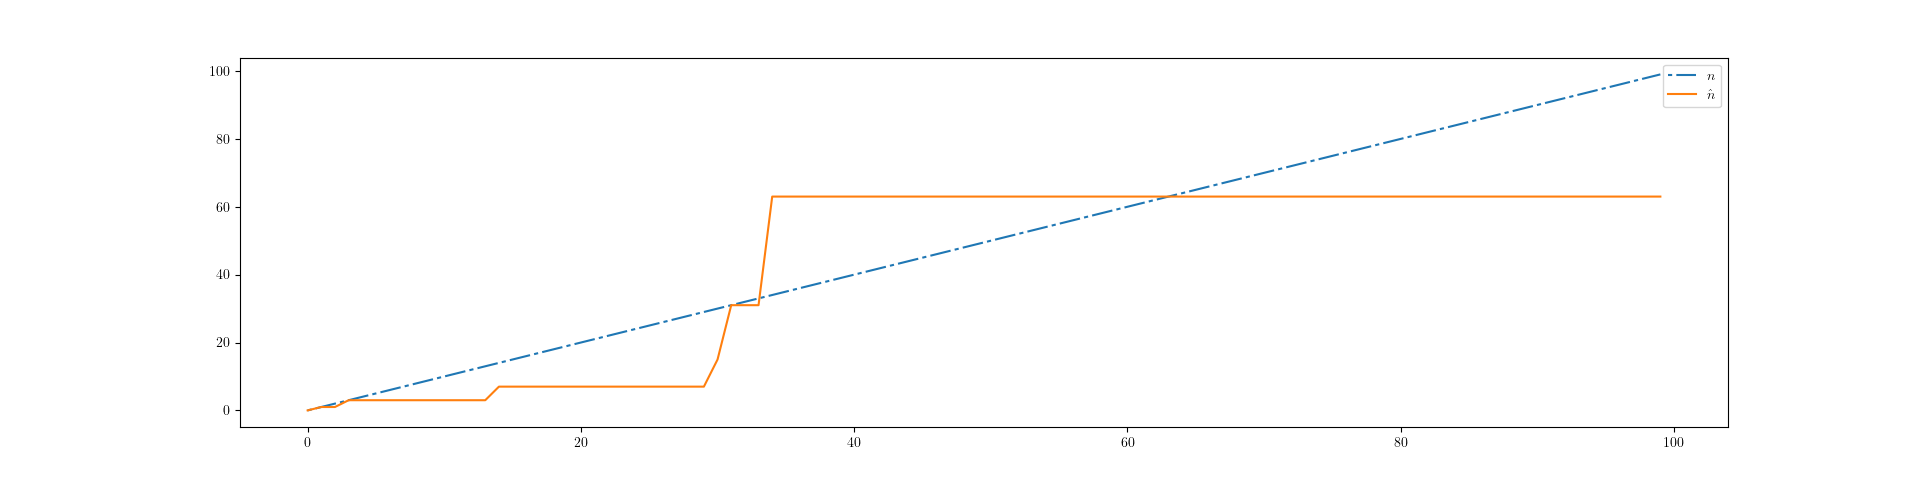
\includegraphics[height=6cm, width=15cm]{figuras/morris_100.png}
	\caption{Simulação do Algoritmo $\Morris$ (100 primeiras iterações)}
  \label{fig:morris:100}
\end{figure}

No entanto, somente com o gráfico acima, pode ser difícil visualizar o erro relativo do algoritmo ao longo das 
iterações. É por isso que construímos também, o gráfico da Figura~\ref{fig:morris:error:100}, em que o eixo x representa 
novamente as iterações da simulação e o eixo y, o erro relativo.

\begin{figure}
  \centering
  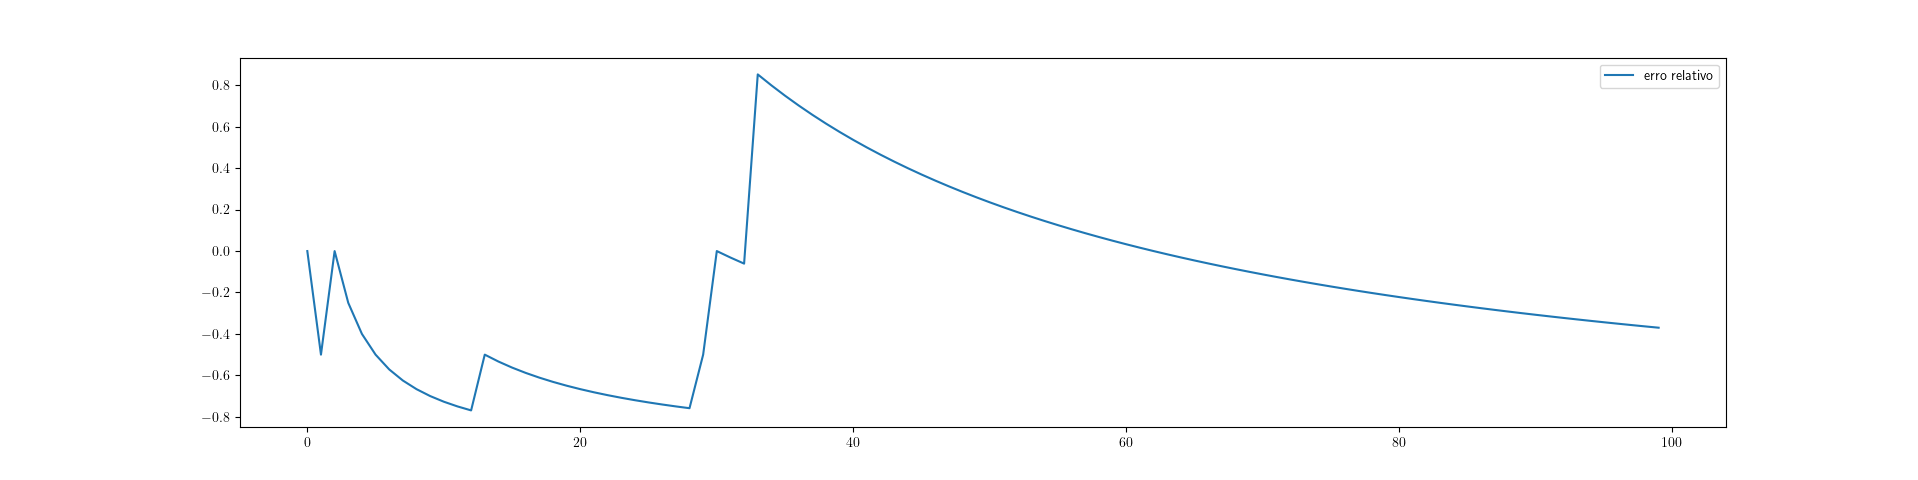
\includegraphics[height=6cm, width=15cm]{figuras/morris_erro_100.png}
	\caption{Erro relativo da simulação do Algoritmo $\Morris$ (100 primeiras iterações)}
  \label{fig:morris:error:100}
\end{figure}

Para as primeiras cem iterações da simulação, é possível perceber pela Figura~\ref{fig:morris:error:100}, que o erro 
relativo não é maior que $0.8$. Na seção sobre a 
\hyperref[sec:morris:analysis]{qualidade da aproximação do Algoritmo $\Morris$}, chegamos à conclusão que o erro 
relativo cometido por $\Morris(\Mbb)$ é quase certamente menor do que 4. Nesse sentido, o pedaço inicial da simulação 
está dentro do esperado. Vamos agora, verificar se esse resultado esperado se mantém conforme mais iterações são 
realizadas.

\begin{figure}
  \centering
  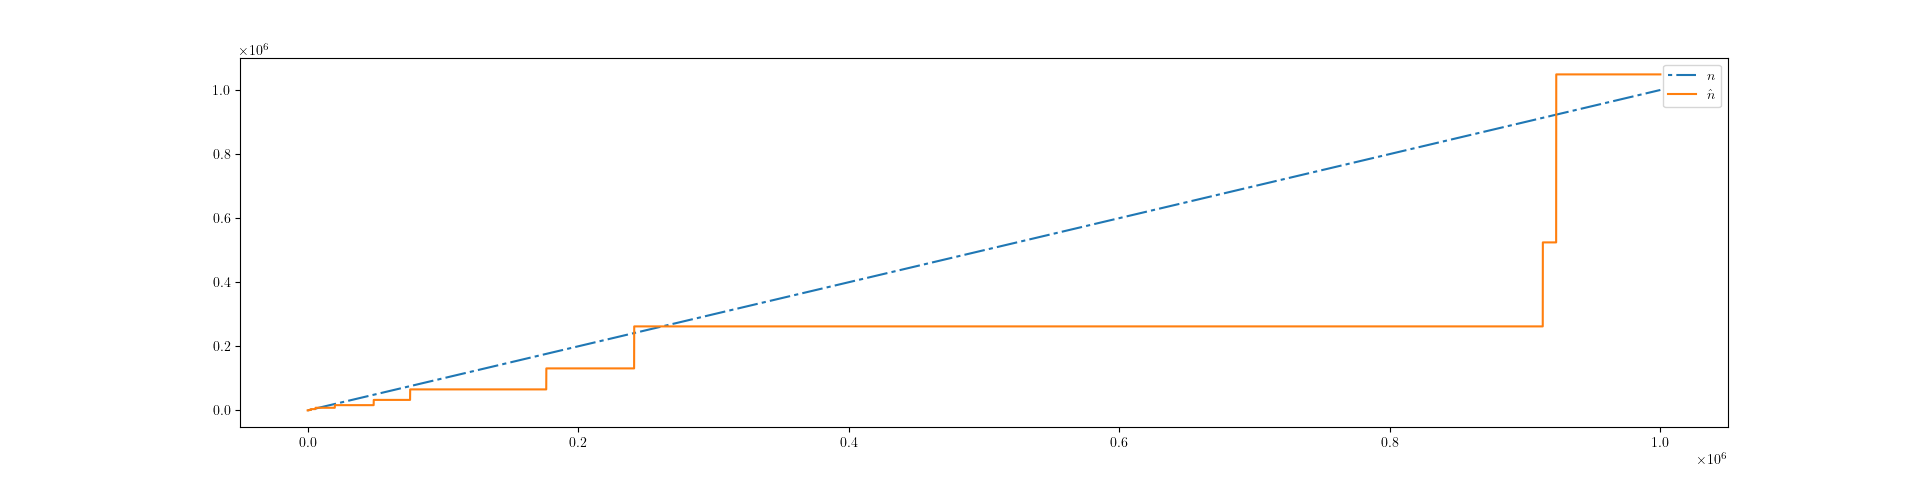
\includegraphics[height=6cm, width=15cm]{figuras/morris_1000000.png}
	\caption{Simulação do Algoritmo $\Morris$ (todas as iterações)}
  \label{fig:morris:1000000}
\end{figure}

\begin{figure}
  \centering
  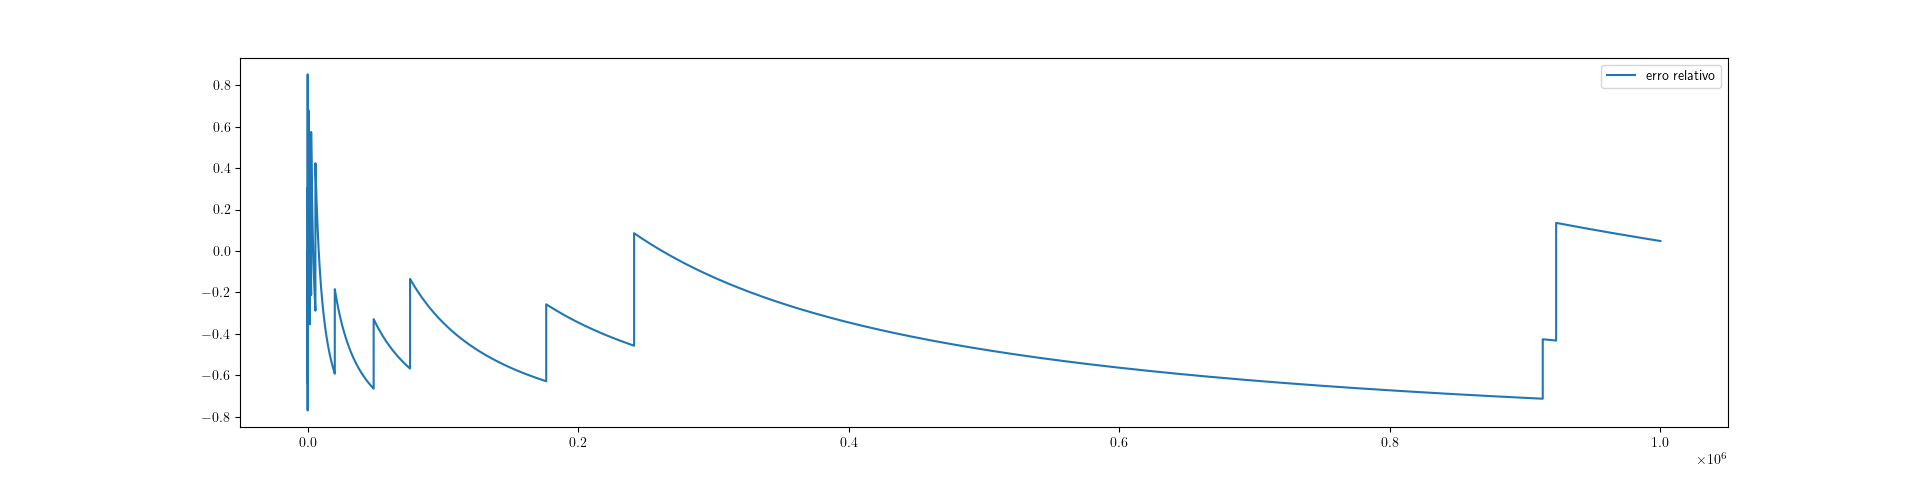
\includegraphics[height=6cm, width=15cm]{figuras/morris_erro_1000000.png}
	\caption{Erro relativo da simulação do Algoritmo $\Morris$ (todas as iterações)}
  \label{fig:morris:error:1000000}
\end{figure}

A Figura~\ref{fig:morris:error:1000000}, que exibe um gráfico com erro relativo ao longo de toda a simulação, nos leva
à conclusão que o erro relativo do algoritmo ficou dentro da faixa esperada (menor que~4). Já a 
Figura~\ref{fig:morris:1000000}, que exibe um gráfico que destaca a evolução da estimativa da quantidade de itens 
inseridos ao longo de toda a simulação, ressalta uma importante característa da estrutura: que quanto mais itens tiverem
sido inseridos, mais demorado é para que a estimativa cresça. Isto está diretamente relacionado com a probabilidade do 
contador~$X$ ser incrementado no Algoritmo~$\Morris$. Contudo, esse incremento demorado não é uma certeza absoluta, uma
vez que, existem casos nesse experimento em que um crescimento da estimativa ocorreu em menos iterações que o 
crescimento anterior. 

Uma dessas situações pode ser vista na Figura~\ref{fig:morris:interval}. Nessa figura, as linhas verticais indicam as 
iterações nas quais o contador foi incrementado. Assim, o contador foi incrementado nas iterações de números 75720, 
176384 e 241343. 

Para que houvesse o incremento na iteração 176384, precisaram ser feitas $176384 - 75720 = 100664$ iterações. Dessa 
forma, esperamos que o próximo incremento aconteça em pelo menos duzentas mil iterações. Só que ele ocorre antes, após 
$241343 - 176384 = 64959$~iterações.

\begin{figure}
  \centering
  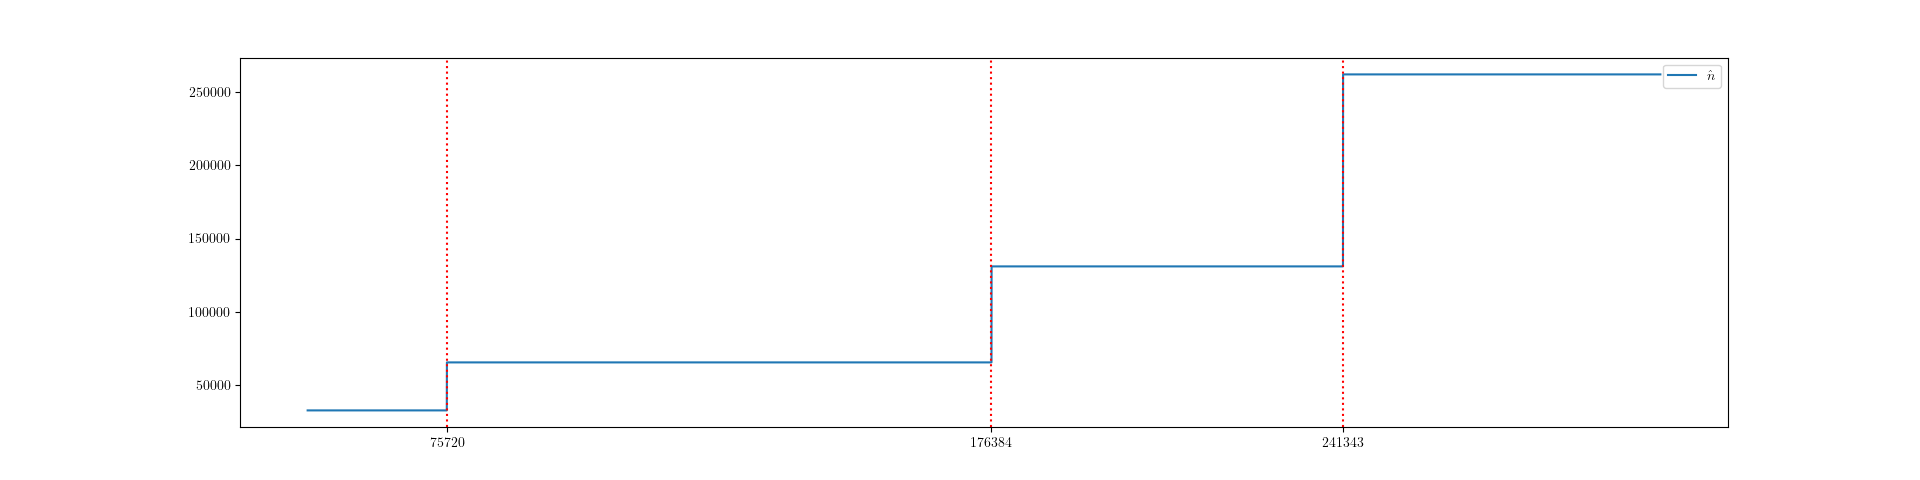
\includegraphics[height=6cm, width=15cm]{figuras/morris_interval.png}
	\caption{Situação em que o contador foi incrementado mais cedo que o esperado. As linhas verticais indicam as 
  iterações nas quais ocorreram um incremento do contador. }
  \label{fig:morris:interval}
\end{figure}
